\documentclass{article}
\usepackage{tikz}
\usepackage{pgfplots}

\begin{document}
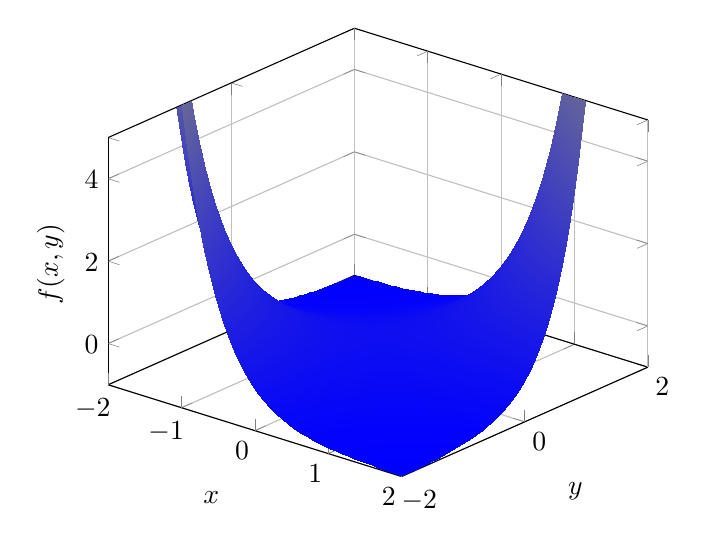
\begin{tikzpicture}
  \begin{axis}[
    xlabel=$x$,
    ylabel=$y$,
    zlabel={$f(x,y)$}, 
    xmin=-2,
    xmax=2,
    ymin=-2,
    ymax=2,
    zmin=-1,
    zmax=5,
    view={40}{30},
    grid=major
  ]
    \addplot3[
      surf,
      domain=-2:2,
      samples=50,
      shader=interp
    ] {exp(x*y) - 1};
  \end{axis}
\end{tikzpicture}
\end{document}